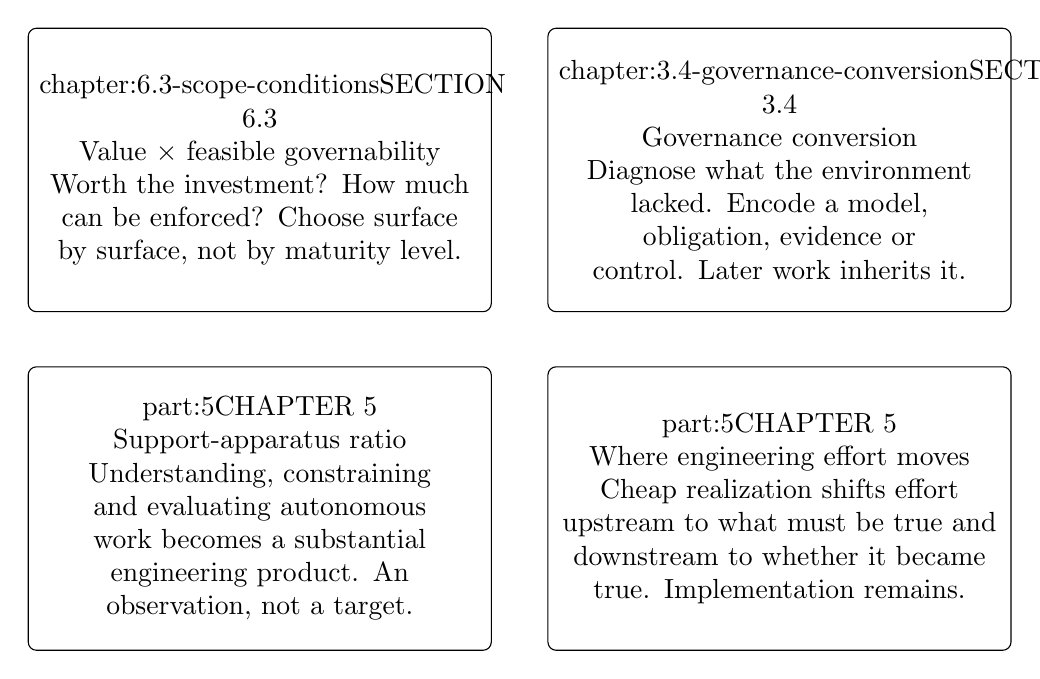
\begin{tikzpicture}[x=1cm,y=1cm,font=\magefigurefont\fontsize{10}{12}\selectfont,
box/.style={draw=black,fill=white,rounded corners=3pt,align=center,text width=3cm,minimum height=8mm,inner sep=4pt},
gate/.style={box,line width=1pt},note/.style={align=center,fill=white,inner sep=1pt,font=\magefigurefont\fontsize{9}{11}\selectfont},
edge/.style={-{Stealth[length=2mm]},line width=.6pt},optional/.style={edge,dashed},
every node/.style={text=black,execute at begin node={\hyphenpenalty=10000\exhyphenpenalty=10000}}]
\node[box,minimum height=36mm,text width=5.6cm] (p0) at (-3.3,0.0) {\magebookref{chapter:6.3-scope-conditions}{SECTION 6.3}\\ Value $\times$ feasible governability\\ Worth the investment? How much can be enforced? Choose surface by surface, not by maturity level.};
\node[box,minimum height=36mm,text width=5.6cm] (p1) at (3.3,0.0) {\magebookref{chapter:3.4-governance-conversion}{SECTION 3.4}\\ Governance conversion\\ Diagnose what the environment lacked. Encode a model, obligation, evidence or control. Later work inherits it.};
\node[box,minimum height=36mm,text width=5.6cm] (p2) at (-3.3,-4.3) {\magebookref{part:5}{CHAPTER 5}\\ Support-apparatus ratio\\ Understanding, constraining and evaluating autonomous work becomes a substantial engineering product. An observation, not a target.};
\node[box,minimum height=36mm,text width=5.6cm] (p3) at (3.3,-4.3) {\magebookref{part:5}{CHAPTER 5}\\ Where engineering effort moves\\ Cheap realization shifts effort upstream to what must be true and downstream to whether it became true. Implementation remains.};
\end{tikzpicture}
